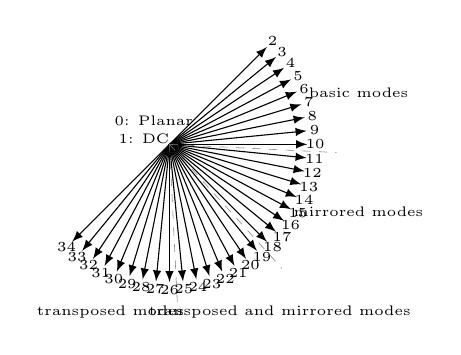
\begin{tikzpicture}[scale=0.5]

	\def\startx{0}
	\def\starty{0}
	\def\radius{3.5}
	\def\startangle{45}
	\def\colour{black}
	\def\style{}

	\draw (-0.4, 0.6) node {\tiny 0: \color{\colour}{\tiny Planar}};
	\draw (-0.65, 0.5) node[below] {\tiny 1: \color{\colour}{\tiny DC}};

	% draw the basic HEVC IPMs with different styles
	\foreach \direction in {2,3,...,34}
	{%
		% set the angle of current prediction direction 
		\pgfmathsetmacro{\angle}{\startangle - (\direction - 2) * 180 / 32}
		% \ifthenelse{\direction = 18}{\def\thickness{very thick}};
		% \ifthenelse{\direction = 26}{\def\thickness{very thick}};
		% basic modes
		\ifthenelse{\direction > 1 \AND \direction < 11}{\def\colour{black}};
		% mirror modes
		\ifthenelse{\direction > 10 \AND \direction < 19}{\def\style{dashed}};
		% transposed and mirrored modes
		\ifthenelse{\direction > 18 \AND \direction < 26}{\def\style{dotted}};
		% transposed modes
		\ifthenelse{\direction > 25 \AND \direction < 35}{\def\style{dashed}};
		% draw the directions
		\draw[-latex,\colour, \style] (\startx,\starty) --++ (\angle:\radius);
		% label each prediction direction
		\draw(\angle:\radius + 0.2) node {\tiny \direction};
	}

	% draw separators
	\foreach \direction in {10, 18, 25}
	{
		\pgfmathsetmacro{\angle}{\startangle - (\direction + 0.5 - 2) * 180 / 32}
		\draw[help lines, dashed] (\startx,\starty) --++ (\angle:\radius + 0.75);
	}

	% label IPM groups
	\draw (4.8,1.3) node {\tiny basic modes};
	\draw (4.8,-1.7) node {\tiny mirrored modes};
	\draw (2.8,-4.25) node {\tiny transposed and mirrored modes};
	\draw (-1.5,-4.25) node {\tiny transposed modes};

\end{tikzpicture}
